\documentclass{article}
\usepackage{amsmath,amssymb,amsfonts}  % For math symbols and fonts
\usepackage{graphicx}                   % For including images
\usepackage{hyperref}                   % For hyperlinks
\usepackage{cite}                       % For citations

\usepackage{algorithm}
\usepackage{algorithmic}

\usepackage{amsthm}
% Define new theorem-like environments
% Define environments
\theoremstyle{definition} % Non-italicized style
\newtheorem{definition}{Definition}[section]
\newtheorem{exercise}{Exercise}[section]

% Title and author info
\title{Makes drones in cirle Experiments Report}
\author{
Zhang Jinrui\thanks{alternative email:zhangjr1022@mails.jlu.edu.cn} \\ \texttt{jerryzhang40@gmail.com}
\\Su Zinan \\ \texttt{suzinan20050803@aliyun.com}
\\Xu Haoran\thanks{alternative email:Xuhr1023@mails.jlu.edu.cn} \\ \texttt{haoranxu288@gmail.com}
}

\date{20250720}  % Empty date; optional, you can also specify a date here

\begin{document}

\maketitle

\begin{abstract}
    In this article, I tried to do apply a
    simple policy to each drone to make
    them fly in cirle
\end{abstract}

\section{recite of the problem \& assumptions}
There are 10 drones and fly on the sky
obeys Newton's second law of motion.
which is
\[
    \vec{F} = m \vec{a}
\]
\[
    \vec{a} = \frac{d\vec{v}}{dt} = \frac{d^2 \vec{x}}{dt^2}
\]
And I mean the policy by, we need a function of force
depending on some communication between drones
to decide the \(\vec{F}\)
\[
    \vec{F}=f(the current information)
\]

And then we want the following dynamic system
\[\begin{bmatrix}
        \frac{d\vec{d}}{dt} \\
        \frac{d\vec{v}}{dt}
    \end{bmatrix}=
    \begin{bmatrix}
        \vec{v} \\
        \vec{a}=f/m
    \end{bmatrix}
\]
has some Self-organized emergent phenomena,
to automatically emergent a circle rounding pattern.

\section{a simple prompt}
To be more clear of the notations we use,
we have \(i\in\{1,2,...,10\}=N\)
And the drones are ignored of its flying
height, which the position vector can be a
2d vector note it as \(\vec{d_i}\)
And so the velocity and acceleration we denote as
\(\vec{v_i}=\frac{d\vec{d_i}}{dt}\)
and
\(\vec{a_i}=\frac{d\vec{v_i}}{dt}\)
I want to prompt a \(f\) so that it can form
a cirle.
\[
    \vec{f_i}=m_i(\sum_{\forall k\neq i,\|\vec{d_i}-\vec{d_k}\|\leq R}(\frac{\vec{d_i}-\vec{d_k}}{\|\vec{d_i}-\vec{d_k}\|^3})+(\frac{\vec{d_{t(i)}}-\vec{d_i}}{\|\vec{d_{t(i)}}-\vec{d_i}\|}-v_i))
\]
This model is easy to explain, the first term is
just a inverse square propell force, the second
term is make the velocity quickly approch a set direction
the \(t(i)\) is just a randomly choosed target drone
other than \(i\) that is \(t(i)\in N, t(i)\neq i\)

This formula can be rewrite without physical term as
follow.
\[
    \vec{a_i}=\sum_{\forall k\neq i,\|\vec{d_i}-\vec{d_k}\|\leq R}(\frac{\vec{d_i}-\vec{d_k}}{\|\vec{d_i}-\vec{d_k}\|^3})+(\frac{\vec{d_{t(i)}}-\vec{d_i}}{\|\vec{d_{t(i)}}-\vec{d_i}\|}-v_i)
\]
separately view this is combined by two independent force
\[
    (\vec{a_i})_{target}=(\frac{\vec{d_{t(i)}}-\vec{d_i}}{\|\vec{d_{t(i)}}-\vec{d_i}\|}-v_i)
\]
\[
    (\vec{a_i})_{propell}=\sum_{\forall k\neq i,\|\vec{d_i}-\vec{d_k}\|\leq R}(\frac{\vec{d_i}-\vec{d_k}}{\|\vec{d_i}-\vec{d_k}\|^3})
\]

\section{a simple prompt:simulation}
\subsection{Four drone case}
\subsubsection{derivation}
This case just choose \(N=\{1,2,3,4\}\)
and don't allow \(t(t(i))=i\)
which definitely form a three element loop and
a dangling drone.

We have a (4,2)-tensor \(\vec{d_i}\)
and two other (4,2)-tensor \(\vec{v_i}\)
and \(\vec{a_i}\)
The initial points are randomly choosed
in Uniformly \([0,1]\times[0,1]\)

choose a time increment \(dt\)
and the simulation update formula is simple to write

just as follow
\[\begin{bmatrix}
        \vec{{d_{n+1}}_i} \\
        \vec{{v_{n+1}}_i}
    \end{bmatrix}=
    \begin{bmatrix}
        \vec{{d_{n}}_i}+\vec{{v_n}_i}dt \\
        \vec{{v_{n}}_i}+(\sum_{\forall k\neq i,\|\vec{{d_n}_i}-\vec{{d_n}_k}\|\leq R}(\frac{\vec{{d_n}_i}-\vec{{d_n}_k}}{\|\vec{{d_n}_i}-\vec{{d_n}_k}\|^3})+(\frac{\vec{{d_n}_{t(i)}}-\vec{{d_n}_i}}{\|\vec{{d_n}_{t(i)}}-\vec{{d_n}_i}\|}-{v_n}_i))dt
    \end{bmatrix}
\]

simple Euler method.
\subsubsection{code \& result}
the computational code are \cite[FourDroneCase]{FourDroneCase} .
the results are shown by the following pictrues which
generated by the code.
The video are \cite[sample1-video]{sample1-video}
and \cite[sample2-video]{sample2-video}
and more other in the same folder on github.
\begin{figure}[ht!]
    \centering
    \begin{minipage}{0.45\textwidth}
        \centering
        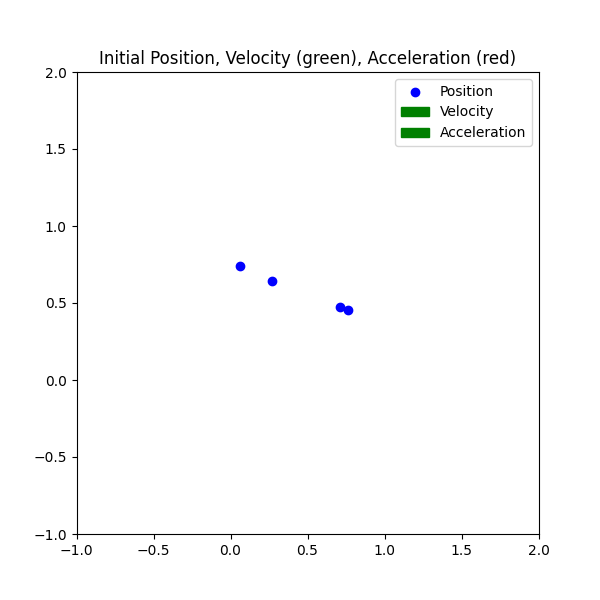
\includegraphics[width=0.9\textwidth]{fig/sample1/dd.png} % first figure itself
        \caption{sample1 randomly initial position}
        \label{fig:fig1}
    \end{minipage}\hfill
    \begin{minipage}{0.45\textwidth}
        \centering
        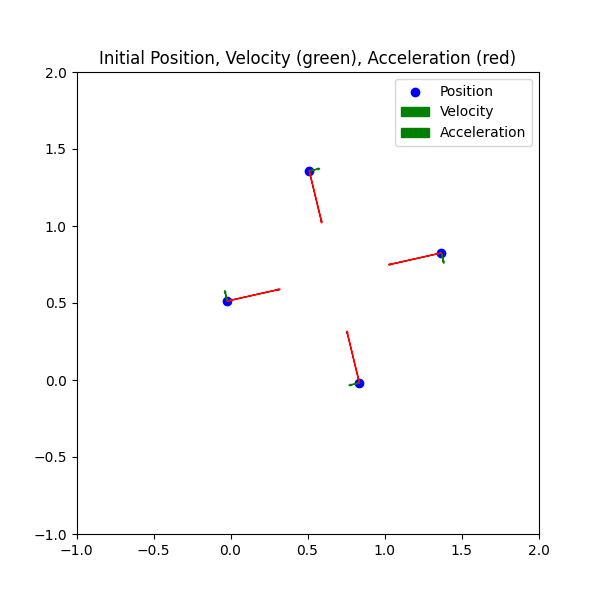
\includegraphics[width=0.9\textwidth]{fig/sample1/dd_18254.png} % second figure itself
        \caption{sample1 after a period of time}
    \end{minipage}
\end{figure}
\begin{figure}[ht!]
    \centering
    \begin{minipage}{0.45\textwidth}
        \centering
        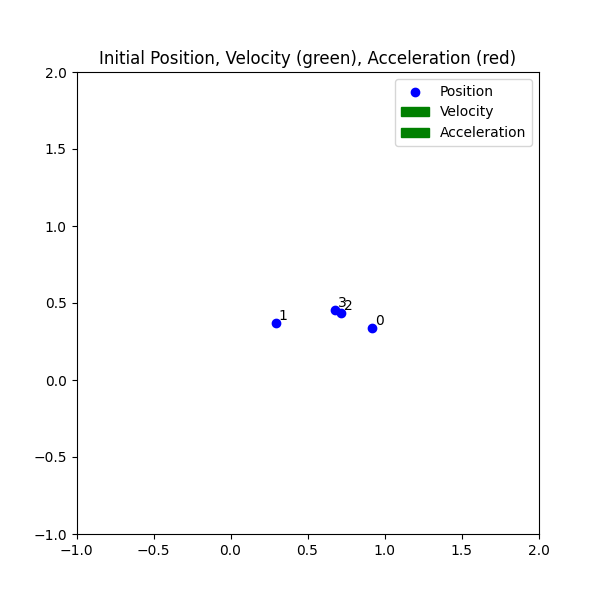
\includegraphics[width=0.9\textwidth]{fig/sample2/dd.png} % first figure itself
        \caption{sample1 randomly initial position}
        \label{fig:fig2}
    \end{minipage}\hfill
    \begin{minipage}{0.45\textwidth}
        \centering
        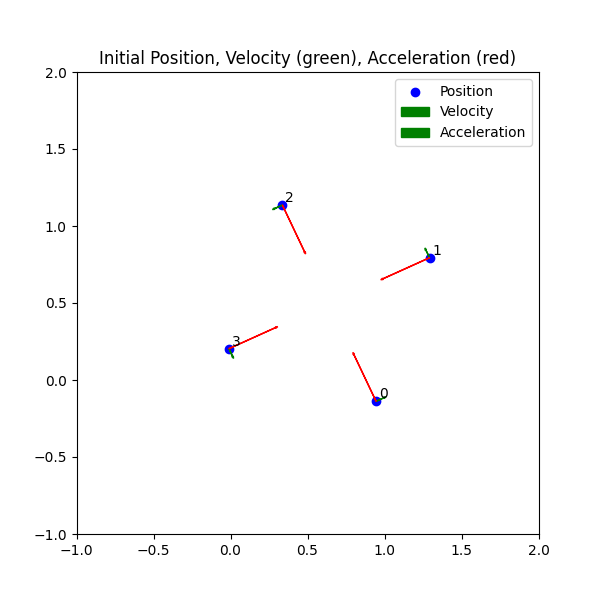
\includegraphics[width=0.9\textwidth]{fig/sample2/dd_18993.png} % second figure itself
        \caption{sample2 after a period of time}
    \end{minipage}
\end{figure}

\subsection{Ten drone case}
undergoing
\subsubsection{derivation}
undergoing

\section{some analysis why it will have a stability property}
\subsection{the terminate radius R}
undergoing
\subsection{the terminate center O}
undergoing
\subsection{graph theory part}
The \(t(i)\) forms a graph which have \(n\) points
and \(n\) oriented edges, this forms a tree with a extra
edges, and this case It will obviously form a Unicyclic Graph.

Which is a tree if we treat all the point on the
loop as the same point.

\section{Zinan Su's approach}
\subsection{notations \& equations}
safe collide radius is \(d_s\)
\[
    \sigma=2d_s
\]
\(NUM\) is the total number of the drones.
And then we want the following dynamic system
\[\begin{bmatrix}
        \frac{d\vec{p_i}}{dt} \\
        \frac{d\vec{v_i}}{dt}
    \end{bmatrix}=
    \begin{bmatrix}
        \vec{v_i} \\
        \vec{a_i}
    \end{bmatrix}
\]
circle origin is a function
\[
    c=\frac{1}{NUM}\sum_{k=1}^{NUM}p_k
\]
Four constants.
\[
    k_p=
\]
\[
    k_d=
\]
\[
    k_v=
\]
\[
    k_r=
\]
\[
    R^*=\frac{1}{NUM}\sum_{k=1}^{NUM}p_k(0)-c(0)
\]
\[
    v_d=\frac{1}{NUM}\sum_{k=1}^{NUM}\|v_k(0)\|
\]
and
\[
    r_i=p_i-c
\]
\[
    d_i=\|r_i\|
\]
\[
    \hat{r_i}=\frac{r_i}{d_i}
\]
\[
    \hat{\theta_i}=\mathbb{M}_\theta r_i
\]
\[
    \mathbb{M}_\theta=
    \begin{bmatrix}
        0  & 1 \\
        -1 & 0
    \end{bmatrix}
\]
\[
    {v_{i}}_{\parallel}=\hat{r_i}\cdot v_i
\]
\[
    {v_{i}}_{\perp}=\hat{\theta_i}\cdot v_i
\]
\[
    U(r)=k_re^{-\frac{r}{2\sigma^2}}
\]
\[
    U_{ij}=U(\|p_i-p_j\|)
\]
\[
    \vec{u_i}_1=[-k_p(d_i-R^*)-k_d{v_{i}}_{\parallel}]\hat{r_i}
\]
\[
    \vec{u_i}_2=[-k_v({v_{i}}_{\perp}-v_d)]\hat{\theta_i}
\]
\[
    \vec{u_i}_3=\sum_{\forall k\neq i}(-\nabla_{p_i}U_{ij})
\]
\[
    \vec{u_i}=\vec{u_i}_1+\vec{u_i}_2+\vec{u_i}_3
\]

\subsection{analysis}
\(c\) is air resistance constant.
\[
    m\frac{d^2 \vec{p_i}}{dt^2}+c\|\frac{d\vec{p_i}}{dt}\|\frac{d\vec{p_i}}{dt}=u_i
\]
\subsection{some constants calculation}
\(c\) is air resistance constant.
\[
    m\frac{d^2 \vec{p_i}}{dt^2}+c\|\frac{d\vec{p_i}}{dt}\|\frac{d\vec{p_i}}{dt}=u_i
\]



\bibliographystyle{plain}  % or another style like unsrt, IEEEtran, etc.
\bibliography{references}  % references.bib is the file name

\end{document}
